

\tikzset{every picture/.style={line width=0.75pt}} %set default line width to 0.75pt        

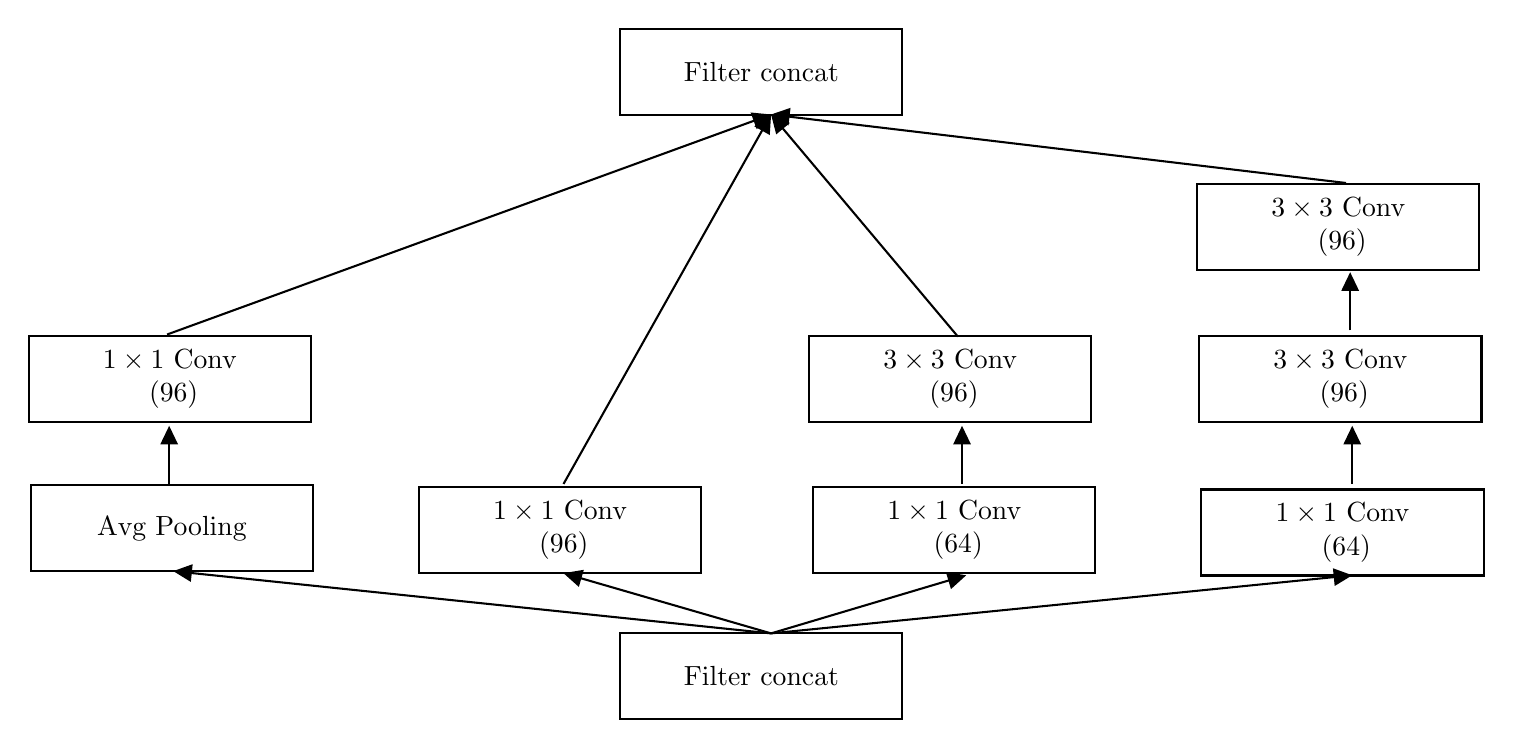
\begin{tikzpicture}[x=0.75pt,y=0.75pt,yscale=-1,xscale=1]
%uncomment if require: \path (0,550.3333358764648); %set diagram left start at 0, and has height of 550.3333358764648

%Flowchart: Process [id:dp8446713243434529] 
\draw   (508,479) -- (643.93,479) -- (643.93,520.43) -- (508,520.43) -- cycle ;
%Flowchart: Process [id:dp8389212433494444] 
\draw   (224,408) -- (359.93,408) -- (359.93,449.43) -- (224,449.43) -- cycle ;
%Flowchart: Process [id:dp9696039225192121] 
\draw   (411,409) -- (546.93,409) -- (546.93,450.43) -- (411,450.43) -- cycle ;
%Flowchart: Process [id:dp31126408548780393] 
\draw   (601,409) -- (736.93,409) -- (736.93,450.43) -- (601,450.43) -- cycle ;
%Flowchart: Process [id:dp739948518816423] 
\draw   (788,410) -- (923.93,410) -- (923.93,451.43) -- (788,451.43) -- cycle ;
%Straight Lines [id:da20227844614554824] 
\draw    (580.67,479.33) -- (294.66,449.54) ;
\draw [shift={(292.67,449.33)}, rotate = 365.95] [fill={rgb, 255:red, 0; green, 0; blue, 0 }  ][line width=0.75]  [draw opacity=0] (8.93,-4.29) -- (0,0) -- (8.93,4.29) -- cycle    ;

%Straight Lines [id:da9079516459586603] 
\draw    (580.67,479.33) -- (482.59,450.89) ;
\draw [shift={(480.67,450.33)}, rotate = 376.16999999999996] [fill={rgb, 255:red, 0; green, 0; blue, 0 }  ][line width=0.75]  [draw opacity=0] (8.93,-4.29) -- (0,0) -- (8.93,4.29) -- cycle    ;

%Straight Lines [id:da7697048902828942] 
\draw    (580.67,479.33) -- (672.75,451.9) ;
\draw [shift={(674.67,451.33)}, rotate = 523.4100000000001] [fill={rgb, 255:red, 0; green, 0; blue, 0 }  ][line width=0.75]  [draw opacity=0] (8.93,-4.29) -- (0,0) -- (8.93,4.29) -- cycle    ;

%Straight Lines [id:da004295071242706339] 
\draw    (580.67,479.33) -- (858.68,451.53) ;
\draw [shift={(860.67,451.33)}, rotate = 534.29] [fill={rgb, 255:red, 0; green, 0; blue, 0 }  ][line width=0.75]  [draw opacity=0] (8.93,-4.29) -- (0,0) -- (8.93,4.29) -- cycle    ;

%Flowchart: Process [id:dp6126721254059377] 
\draw   (223,336) -- (358.93,336) -- (358.93,377.43) -- (223,377.43) -- cycle ;
%Flowchart: Process [id:dp6415327260036892] 
\draw   (599,336) -- (734.93,336) -- (734.93,377.43) -- (599,377.43) -- cycle ;
%Flowchart: Process [id:dp557242506777897] 
\draw   (787,336) -- (922.93,336) -- (922.93,377.43) -- (787,377.43) -- cycle ;
%Flowchart: Process [id:dp895045490145193] 
\draw   (786,263) -- (921.93,263) -- (921.93,304.43) -- (786,304.43) -- cycle ;
%Straight Lines [id:da042686267300120706] 
\draw    (290.67,407.33) -- (290.67,381.33) ;
\draw [shift={(290.67,379.33)}, rotate = 450] [fill={rgb, 255:red, 0; green, 0; blue, 0 }  ][line width=0.75]  [draw opacity=0] (8.93,-4.29) -- (0,0) -- (8.93,4.29) -- cycle    ;

%Straight Lines [id:da1451751743173857] 
\draw    (672.67,407.33) -- (672.67,381.33) ;
\draw [shift={(672.67,379.33)}, rotate = 450] [fill={rgb, 255:red, 0; green, 0; blue, 0 }  ][line width=0.75]  [draw opacity=0] (8.93,-4.29) -- (0,0) -- (8.93,4.29) -- cycle    ;

%Straight Lines [id:da7065201039263691] 
\draw    (860.67,407.33) -- (860.67,381.33) ;
\draw [shift={(860.67,379.33)}, rotate = 450] [fill={rgb, 255:red, 0; green, 0; blue, 0 }  ][line width=0.75]  [draw opacity=0] (8.93,-4.29) -- (0,0) -- (8.93,4.29) -- cycle    ;

%Straight Lines [id:da3529249322466719] 
\draw    (859.67,333.33) -- (859.67,307.33) ;
\draw [shift={(859.67,305.33)}, rotate = 450] [fill={rgb, 255:red, 0; green, 0; blue, 0 }  ][line width=0.75]  [draw opacity=0] (8.93,-4.29) -- (0,0) -- (8.93,4.29) -- cycle    ;

%Flowchart: Process [id:dp023795399666625805] 
\draw   (508,188) -- (643.93,188) -- (643.93,229.43) -- (508,229.43) -- cycle ;
%Straight Lines [id:da14696140485542641] 
\draw    (289.67,335.33) -- (578.79,230.02) ;
\draw [shift={(580.67,229.33)}, rotate = 519.99] [fill={rgb, 255:red, 0; green, 0; blue, 0 }  ][line width=0.75]  [draw opacity=0] (8.93,-4.29) -- (0,0) -- (8.93,4.29) -- cycle    ;

%Straight Lines [id:da7335126004687851] 
\draw    (480.67,407.33) -- (579.69,231.08) ;
\draw [shift={(580.67,229.33)}, rotate = 479.33] [fill={rgb, 255:red, 0; green, 0; blue, 0 }  ][line width=0.75]  [draw opacity=0] (8.93,-4.29) -- (0,0) -- (8.93,4.29) -- cycle    ;

%Straight Lines [id:da6191146997492387] 
\draw    (670.67,336.33) -- (581.95,230.86) ;
\draw [shift={(580.67,229.33)}, rotate = 409.93] [fill={rgb, 255:red, 0; green, 0; blue, 0 }  ][line width=0.75]  [draw opacity=0] (8.93,-4.29) -- (0,0) -- (8.93,4.29) -- cycle    ;

%Straight Lines [id:da444168686885831] 
\draw    (857.67,262.33) -- (582.65,229.57) ;
\draw [shift={(580.67,229.33)}, rotate = 366.78999999999996] [fill={rgb, 255:red, 0; green, 0; blue, 0 }  ][line width=0.75]  [draw opacity=0] (8.93,-4.29) -- (0,0) -- (8.93,4.29) -- cycle    ;


% Text Node
\draw (575.96,499.71) node  [align=left] {Filter concat};
% Text Node
\draw (291.96,428.71) node  [align=left] {Avg Pooling};
% Text Node
\draw (478.96,429.71) node  [align=left] {$\displaystyle 1\times 1$ Conv\\ \ \ \ \ \ (96)};
% Text Node
\draw (668.96,429.71) node  [align=left] {$\displaystyle 1\times 1$ Conv\\ \ \ \ \ \ (64)};
% Text Node
\draw (855.96,430.71) node  [align=left] {$\displaystyle 1\times 1$ Conv\\ \ \ \ \ \ (64)};
% Text Node
\draw (290.96,356.71) node  [align=left] {$\displaystyle 1\times 1$ Conv\\ \ \ \ \ \ (96)};
% Text Node
\draw (666.96,356.71) node  [align=left] {$\displaystyle 3\times 3$ Conv\\ \ \ \ \ \ (96)};
% Text Node
\draw (854.96,356.71) node  [align=left] {$\displaystyle 3\times 3$ Conv\\ \ \ \ \ \ (96)};
% Text Node
\draw (853.96,283.71) node  [align=left] {$\displaystyle 3\times 3$ Conv\\ \ \ \ \ \ (96)};
% Text Node
\draw (575.96,208.71) node  [align=left] {Filter concat};


\end{tikzpicture}